\documentclass[12pt,a4paper,leqno]{report}

\usepackage[T1]{fontenc}
\usepackage[english]{babel}
\usepackage{amsthm}
\usepackage{amsfonts}
\usepackage{amsmath}
\usepackage{amssymb}
\usepackage{tikz}

\newcommand{\R}{\mathbb{R}}
\newcommand{\C}{\mathbb{C}}
\newcommand{\Q}{\mathbb{Q}}
\newcommand{\N}{\mathbb{N}}
\newcommand{\No}{\mathbb{N}_0}
\newcommand{\Z}{\mathbb{Z}}
\newcommand{\diam}{\operatorname{diam}}

\theoremstyle{plain}
\newtheorem{equa}[equation]{Equation}
\newtheorem{lem}[equation]{Lemma}
\newtheorem{prop}[equation]{Proposition}
\newtheorem{cor}[equation]{Corollary}

\theoremstyle{definition}
\newtheorem{defi}[equation]{definition}
\newtheorem{conj}[equation]{Conjecture}
\newtheorem{example}[equation]{Example}

\theoremstyle{remark}
\newtheorem{note}[equation]{Note}

\pagestyle{plain}
\setcounter{page}{1}
\addtolength{\hoffset}{-1.15cm}
\addtolength{\textwidth}{2.3cm}
\addtolength{\voffset}{0.45cm}
\addtolength{\textheight}{-0.9cm}

\title{Applying Bayesian Hierarchical Models to N-of-1 Trials}
\author{Tuomo Kareoja}
\date{27/06/19}

\begin{document}

\maketitle

\tableofcontents

\section{Introduction}\label{intro}

N-of-1 trials in clinical practice are multiple crossover trials conducted on
a single patient, where treatment periods with different treatments are formed
into multiple blocks each of which contains at least one period of each treatment
under consideration\cite{nof1}. By comparing the measurements taken during
different treatments, a comparisons between treatment options can be
made and the most suitable treatment option chosen for the particular patient in question.

In the following pages I give a concise explanation of the experimental design
of N-of-1 trials and how we can statistically model these kinds of experiments
given the kinds of challenges their design poses.
I then follow up with a how we can apply Bayesian methods in estimating the
effectiveness of different treatments highlighting how these methods can gives us
needed flexibility when running N-of-1 trials by not relying on hypothesis testing
depending on a prespecified design. I then consider the case when there are
multiple similar N-of-1 trials and show how it is possible to pool the
information from these with hierarchical Bayesian methods, without loosing
sight of the goal of N-of-1 trials: to find the best
treatment most suitable for each patients particularities.
Finally I end by with a complete example of analyzing multiple N-of-1
trials with hierarchical Bayesian methods using RStan-package with simulated
data.

\chapter{What Are N-of-1 Trials?}\label{nof1}

In the appraisal of any medical treatment the ``gold standard'' is a randomized
controlled trial (RCT), where subjects are randomized to two or more groups
that are given different treatments or no treatment at all. The measurement
from theses groups are then compared and a result derived about which treatment
is most effective on average. This design takes into account unknown factors
that might make some patients more suspectable to one treatment by forming the
groups randomly and thus, on average, distributing these patients evenly
between groups. By comparing the groups against each other and not just to the
same patients at the beginning and end of the study, it also takes into account
time related effects like natural progression of disease. Despite its
unquestionable value in finding general effects, this method can run into problems
when we actually try to apply its results to individual patients in practice.

Knowing the best treatment in average might not help much in finding right
treatment for a particular patient if the variability in treatment
effectiveness between patients is high. Although we can use covariates like
age, gender, or certain gene variant to explain the variance between patients
in RCT:s, there usually is still much unexplained variance. Some of this
variance is of course caused by random factors like measurement error, but a
significant part might be caused real and significant differences between the
patients. In other words, there might be significant factors that explain the
variability of the efficacy of different treatments between patients that
might either be too specific to be considered in a RCT study or unknown and
thus impossible to analyze in this kind of experimental design.

Another problem with RCT:s is the peculiarity of their participants. It is common
practice to accept patients to RCT:s only if they don't suffer from any
medical issue besides the one that is being studied. This lack of comorbidity
makes it easier to get clear results by removing confounding factors, but at
the same time this lowers the external validity of the results, because in the
real world patients often suffer from multiple medical issues simultaneously.
Because of this it might be possible that, even when the scientific literature
provides clear results about the relative effectiveness of different treatments, these
results don't actually generalize that well to the kinds of patients the clinical
practitioner sees in her office.

N-of-1 trials can be used to patch the holes in the knowledge that RCT:s cannot fill by
changing the focus of the study from group averages to individual patient. In N-of-1
design multiple treatments are tried sequentially in periods that are
formed into blocks each of which contains a treatment period of each treatment option
under consideration at least once. Within each treatment period the effects of the
treatments are measured in comparable ways. Depending on the ease of measuring the outcome
of interest, the measurements could be done just once per treatment period,
or even multiple times per day. Each block includes a period of each treatment under
consideration in random or balanced order to take into account time related
effects. A simple example would be a ABBA design that includes two blocks with
which the two treatments A and B are assigned in a balanced order. Depending on
the treatments considered, there might be also be a so called ``washout'' period
between treatments, where the patient does not receive any treatment and her state is
allowed to return to baseline. This method is used to prevent treatment
interactions, that could make it difficult to analyze the results or could be
dangerous to the patient. If the treatments under study allow, N-of-1 trial can
also use the double-blind method, where the patient and caregiver both don't know
which treatment is currently used and placebo treatment, where one of the
treatments only resembles treatment, but does not contain any active
ingredient (pharmacological or otherwise). Below is schema of a more complex
N-of-1 trial with three treatments A, B and C, random assignment of treatments within
blocks, three measurements within each treatment period and a washout periods between treatments:

\bigskip
{
    \centering
    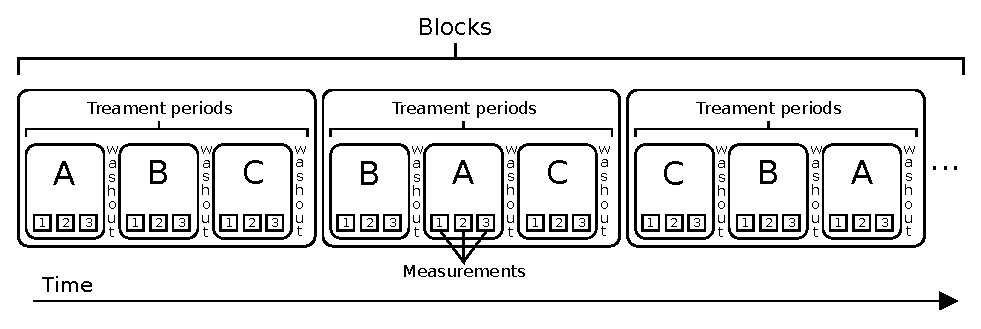
\includegraphics{n-of-1_schema.eps}
    \par
}
\bigskip

The stated aim of N-of-1 trials is quite different from RCT:s: where the latter
tries to generalize results to population and find which treatment is best in
general, the N-of-1 trial tries to only generalize to the patient in question.
This means that where as comorbidity and other factors that cause
systematic variation between the patients in treatment outcomes are a problem
in RCT:s, these are not an issue in N-of-1 trials because there is no need to
generalize beyond the one patient. There is also no actual need to know
what is the factor causing a certain treatment to work better or worse, as long
as it is not because of measurement errors or time related effect.

Use of N-of-1 trials is appropriate in situations where there are multiple
treatment options but there is no prior knowledge of which of these would be
best, when there is known to be considerable variability between patients in
treatment efficacy, or when there is reason to doubt that the results from
scientific literature generalize to the patient in question. This would seem to
make n-of-1 trials applicable to quite a few situations, but there are also
multiple factor restricting their use.

Firstly, N-of-1 trials can only be used on illnesses that are chronic, progress
slowly and are at least somewhat stable. Also the treatments options available
must have a noticeable treatment responses within a short timeframe. This is because
running the trial needs time to complete and fast changing illness or slowly effecting
treatment make it either impossible to distinguish true effects from the natural progression
of the disease or make the trials impracticably lengthy. N-of-1 trials are also unsuitable for
testing of preventative treatments because the effects of these
treatments are often also impossible to measure without comparisons to other
patients without the same treatment.

Secondly, running a N-of-1 trial is costly because of added expenses of training the
medical staff in the method, running the trial with all its measurements and analyzing
the data. This is means that it can be hard to find cases where using this method is
cost effective and studies making these kind calculations have come to pessimistic
conclusions (1,2).

These limitations have kept the use of N-of-1 trials rare in clinical use,
even though they could potentially both increase the life quality of the patients
and lower the healthcare costs by finding most suitable medications to patients that
might end up potentially using them for years. This state of affairs might
be changing fast though. Aging and environmental factors are changing worlds
disease burden so that bigger and bigger proportion of it is constituted by
chronic diseases (3), of which common ones like non-acute
cardiovascular diseases and diabetes are excellent candidates for N-of-1
trials. Also the cost of administering N-of-1 trials are dropping with advent of
cheap and reliable health sensors like smartwatches and connected blood
pressure monitors. For example in diabetic patients it is now possible to get
real time readings of blood insuline levels with minimal effort from the
patient (4). These factors mean that the popularity of this method could potentially
rise significantly in the future.

\chapter{Statistical Modeling of N-of-1 Trials}\label{modeling}

Even though the data created by the N-of-1 trials resembles traditional time
series data with autocorrelation between observations and repeated measurements
from the same study unit, there are additional complexities that are caused by the
structure of repeating treatment periods. Trying to take into account all the
peculiarities of the study design could end up with model too complicated to
the small amount of data generated by a single study, so one must consider
carefully what factors actually need to incorporated in to the model.

Simplest model that we could employ is to just count the number of
blocks where a treatment is considered ``better'' than others. The precise
definition of ``better'' doesn't matter here. This way we arrive to a simple binomial
model where the number of ``successes'' \(X\) is the number of blocks where a treatment
is considered the ``best'' one follows binomial distribution and the probability of
each treatment option of having \(k\) successes is given by:

\begin{def}\label{binom}
\begin{equation}
P(X = k) = {n\choose k}p^k{(1-p)}^{(n-k)}
\end{equation}
\end{def}
, where \(k\) = number of blocks, where the treatments is considered the ``best'',
\(n\) = total number of blocks and \(p\) = the probability of being considered the ``best''.

This type of model is rudimentary at best, because it fails to consider the magnitude of the
differences between treatment effects and does not take into account the actual number of
measurements within each treatment period. To take these factors into account
more complex models are in order.

\section{Basic Models}\label{conti}

Before going further I make the assumption that the measurements are continuous as
this is probably the most common case. Lets first look at a model where we assume
that there are no time-trends and no autocorrelation between measurements.
Let \(y_{mbpt}\) represent the outcome measured while on treatment \(m\) within
treatment block \(b\) within treatment period \(p\) at time \(t\). The treatment
periods are indexed within each block and time is indexed within each treatment
period:

\begin{def}\label{allerrors}
\begin{equation}
y_{mbpt} = \mu_m + \gamma_b + \delta_{p(b)} + \epsilon_{t(p(b))}
\end{equation}
\end{def}
, where \(\gamma_b \sim N(0,\sigma^2_{\gamma})\),
\(\delta_{p(b)} \sim N(0,\sigma^2_{\delta})\), and
\(\epsilon_{t(p(b))} \sim N(0,\sigma^2_{\epsilon})\)

This model assumes all treatment effects \(\mu_m\) to be constant. Between the normally
distributed terms \(\gamma_b\) represents random block effects, \(\delta_{p(b)}\)
random period effects and \(\epsilon_{t(p(b))}\) random within period errors. We could choose one
of the blocks as a reference and set \(\gamma_1 = 0\) and assume that within each block
the between period effects follow a same pattern, e.g.\ the difference between treatment
period one and two is the same within each block.

The random effects between blocks and treatment periods could represent for example the
random variations in the motivation of the patient and possible changes in treating
personnel within each block and treatment period. The random within period errors represents
the measurement error of a single measurements within treatment periods. The relative sizes
of the these terms are important for effective design of the trial because they determine
if it is more be beneficial for the statistical power of the study to add more measurements,
treatment periods or blocks.

If the measurements within blocks and within periods do not correlate, the model 3.2
can be simplified by dropping \(\gamma_b\) and \(\delta_{p(b)}\):

\begin{def}\label{oneerror}
\begin{equation}
y_{mbpt} = \mu_m + \epsilon_{t(p(b))}
\end{equation}
\end{def}
, where \(\epsilon_{t(p(b))} \sim N(0,\sigma^2_{\epsilon})\)

This simple model is a natural fit in scenarios where there is just one measurement within each
treatment period.

\section{Incorporating time-trends into the model}\label{timetrends}

As the symptoms of the patient might not be completely stable (e.g.\ because symptoms get
worse with the progression of the disease) fitting some kind of time-trend to the model
might be advisable. We can modify the model 3.3 from previous chapter to include a linear
time-trend by adding an intercept and slope of the time-trend. In this case
the model can expressed more concisely just in terms of the measurement \(y_t\) taken at time \(t\),
where time is indexed from the start of the experiment:

\begin{def}\label{quadratictimetrend}
\begin{equation}
y_t = \beta_0 + \beta_1 t + \mu_t + \epsilon_t
\end{equation}
\end{def}
, where \(\epsilon_t \sim N(0,\sigma^2)\)

Here \(\beta_0\) is the intercept, \(\beta_1\) the slope of the time trend, \(\mu_t\) the
effect of the treatment given during time \(t\) and \(\epsilon_t\) is the residual error at time \(t\).
More complex time-trends can be introduced by modifying the slope, for example by adding the term
\(\beta_2 t^2\) to introduce a quadratic trend.

Another effect dependent on time to take into consideration are period effects.
There might be some part of the trial that is within a period that we presume to
have its own effect. An example of this kind of effect is if we study asthma
medications and part of the trial falls within the pollen season. A simple way to model this
is to use a dummy variable that takes the value 1 within the period and 0 outside it.
Extending the model 3.4 with a period of constant effect \(\beta_2\) we end up with:

\begin{def}\label{quadratictimetrend}
\begin{equation}
y_t = \beta_0 + \beta_1 t + \beta_{2}Z_t + \mu_t + \epsilon_t
\end{equation}
\end{def}
, where \(\epsilon_t \sim N(0,\sigma^2)\) and dummy variable \(Z_t = 1\)
when \(t \in (t_{period\,start} \ldots t_{period\,end}) \) and \(0\) otherwise.

Lastly, to take into account that treatment effects themselves can vary with time, for example because
treatment works better during periods of greater disease severity, we can add a time-by-treatment
interaction effect into the model. For example in the case where we expect that the
illness gets steadily (e.g.\ linearly) worse with time, but the treatments compensate this
by being similarly more effective, we can extend the model 3.4 that includes a simple
linear time-trend by adding an interaction term \(\mu_t\beta_1 t\):

\begin{def}\label{lineartimetrendwithinteraction}
\begin{equation}
y_t = \beta_0 + \beta_1 t + \mu_t + \mu_t\beta_1 t + \epsilon_t
\end{equation}
\end{def}
, where \(\epsilon_t \sim N(0,\sigma^2)\)

\section{The Problem of Autocorrelation}\label{autocor}

A common occurrence in time-series data is the autocorrelation between
measurements, so that there is similarity between observations defined by
a function of time lag between them. A common first response to this problem
is to add a time-trend to the model like we did in the previous chapter.
This detrending often removes a substantial proportion of the autocorrelation
that could be caused for example by the natural progression of disease or seasonal
variations in its symptoms\cite{stat}. Unfortunately in N-of-1 trials the problems of carryover effects and
slow onset of treatment effect can lead to very complex autocorrelation patterns
that are hard to remove with simple time-trend.

Carryover effects refer to the lingering effects of the treatment even after it has
beed stopped. This can make the treatment effects in next treatment period with
a different treatment seem larger (or smaller in the unfortunate and hopefully rare case
where the previous treatment was actually harmful) than they actually are. Carryover effects also
encompass the effects of interactions between sequential the treatments, which could
even be dangerous depending on the nature of the treatments. On the other hand treatment
effects that manifest slowly can often give the opposite effect of carryover effects by making
the treatments look less effective than they really are during the first measurements of
each treatment period.\cite{stat}

To deal with these more devious sources of autocorrelation in our model we can take two routes.
To make expressing the following models easier I assume here that the time between measurements
is roughly constant and so we can index the time so that each measurement is separated by one
time unit. First possible solution to autocorrelation is to use an autoregressive model where
we express the measurement error at time \(t\) as function of one or more previous measurement errors:

\begin{def}\label{autoregression}
\begin{equation}
y_t = \mu_t + \epsilon_t
\end{equation}
\end{def}
, where \(\epsilon_t = \rho\epsilon_{(t - 1)} + \mu_t\) in which
\(\mu_t\) is the effect of the treatment given at time t,
\(\rho \) is the correlation between consecutive errors and
\(\epsilon_{t-1} \sim N(0,\sigma^2) \) is the error term at \(t-1\).

Instead of making the error dependent on just the previous error the model can be adjusted
to include more complex lag by defining \(\epsilon_t = \rho_1\epsilon_{t-1} +
\rho_2\epsilon_{t-2} + \ldots + \rho_x\epsilon_{t-x} + \mu_t\), where \(\rho_x\) is the correlation
between the errors separated by \(x\) time units (e.g.\ measurements).

Second approach is to use a dynamic model where we express the autocorrelation in the measurements
themselves so that the measurement at time \(t\) is a function of the measurement at \(t-1\):

\begin{def}\label{dynamicmodel}
\begin{equation}
y_t = \rho y_{t-1} + \mu_t + \epsilon_t
\end{equation}
\end{def}
, where \(\mu_t\) is the effect of the treatment given at time \(t\), \(\rho \) is the correlation
between consecutive measurements and \(\epsilon_t \sim N(0,\sigma^2)\) is the error term.

Although it can make more intuitive sense to the make whole observation dependent on
the previous observation, it is important to recognize that in this case the treatment effects
\(\mu_t\) must be interpreted differently as they are now conditioned on the these measurements.

Although we can try to solve problems created by carryover effect and slow manifestation
of treatment effect with modelling, a better way could be to take
measures to mitigate the effects in the study design itself. By having long
enough washout period between different treatments we can minimize the carryover effect. If
there are no harmful interactions between the treatment the next treatment
can be started within the washout period so that we minimize the problem of
slow treatment effects. If there are interactions to be taken into
consideration, the first few measurement at the beginning of
each treatment period could also just be dropped. By doing this we are of course
throwing away data, but we must be remember that if the measurements at the
beginning of the treatment period are mangled, this will also mangle our parameter estimates.
Trying to take these effects into account in our model will probably not eliminate these
effects completely and will increase the complexity of our model.

\section{Non-continuous Measurements}\label{noncontinuous}

Up to this point I have assumed that the measurement used are continuous, but we
could of course have measurements that are binary, counts of events or categorical.
With these kind of measurement the models need reformatting so that they don't
presume normal distributions. Despite this the models still don't have to differ much
from the models presented above and the principals covered before can be applied.

To modify previously presented models to work when measurements are not continuous, we need to to formulate them
as generalized linear models. We do this by keeping the right-hand sides in the same form but expressing the left-hand
side in terms of link function of the mean of the probability distribution of the outcomes.
So instead of expressing the model in terms
of individual observations \(y_t\), we express it as the expected value of these measurements conditional
on the data (and experimental design, because this decides which treatment is given at which point in the experiment)
\(E(Y|D)\) that we feed to the link function.
The link function allows us to model measurements with arbitrary distributions, as now the link function can linearly depend on the parameters of the model,
rather than needing the measurements themselves to do so. We need to do this to prevent the models from giving impossible predictions,
e.g.\ negative counts or probabilities of under 0 or over 1.

Lets work with an example of a binary outcome measurements. In this case the measurements \(y\) at time \(t\) follow the Bernoulli distribution \(y_t \sim Bernoulli(p)\)
where the the expected value of the distribution is the probability \(p\) of observing the event in measurement \(y_t\). In this case the suitable link function is the logit
function \(logit(p)=\log_e(\frac{p}{1-p})\). With this information we can now formulate a simple model with a linear time trend:

\begin{def}\label{oneerror}
\begin{equation}
\log_e(\frac{p_t}{1-p_t})=\beta_0 + \beta_1 t + \mu_t
\end{equation}
\end{def}
, where \(p_t\) is the the probability of observing the event at time \(t\) and \(\log_e(\frac{p_t}{1-p_t})\) are the log-odds of this event,
\(\beta_0\) is the intercept, \(\beta_1\) the slope of the time trend and \(\mu_t\) the
effect of the treatment given during time \(t\).

By first exponentiating (3.10) and then using simple algebraic manipulation we can
express the model in terms of of the probability \(p_t\) (3.11):

\begin{def}\label{oneerror}
\begin{equation}
\frac{p_t}{1-p_t}=e^{\beta_0 + \beta_1 t + \mu_t}
\end{equation}
\end{def}

\begin{def}\label{oneerror}
\begin{equation}
p_t=\frac{e^{\beta_0 + \beta_1 t + \mu_t}}{e^{\beta_0 + \beta_1 t + \mu_t}+1}=\frac{1}{1+e^{-(\beta_0 + \beta_1 t + \mu_t)}}
\end{equation}
\end{def}

We notice that there are no error terms in this model. This is because we are not modelling individual observations,
but the expected value of these values (probability of observing the event under treatment used at time \(t\) in this case). Even though there is random variations in
the individual observations, when we talk about the their expected value
there is just a single value with no random errors. Apart from this difference we can see that we find the same model
from the denominator that we used when modelling a continuous measurement with a linear time-trend in equation 3.4.
This means that to build the models described before, we would just insert the right side of the equations
into the denominator, apart from the error term.

With numbers of events as measurements, instead of expressing the model in terms of time, we can
express it in terms of periods \(p\) that are of equal length and indexed from the beginning of the experiment.
The number of events during period \(p\)
follows a Poisson distribution \(y_p \sim Poisson(\lambda)\)
and the expected value of the distribution is the rate \(\lambda_p \) of the events during period \(p\).
For link function we use the natural log
that is we have \(\log_e(\lambda_p)\) on the left side of the equation.
Once again using the same simple model with linear time trend we end up with a model:

\begin{def}\label{oneerror}
\begin{equation}
\log_e(\lambda_p)=\beta_0 + \beta_1 r + \mu_{p}
\end{equation}
\end{def}
, where \(\lambda_p\) is the the rate of events between measurements during period \(p\),
\(\beta_0\) is the intercept, \(\beta_1\) the slope of the time trend and \(\mu_p\) the
effect of the treatment given during period \(p\). By simply exponentiating both sides
we can express the model in terms of rate of events:

\begin{def}\label{oneerror}
\begin{equation}
\lambda_t=e^{\beta_0 + \beta_1 t + \mu_t}
\end{equation}
\end{def}
, where we now have the familiar linear model formula in the exponent on the right side of
the equation.

The case of categorical measurements is more complex as there are multiple possible link functions
depending on which way we want to model the measurements. Because of this so we don't go trough all of them here.
The one that is probably the most relevant is the case when categorical measurements
are ordinal, that is they have a natural ordering (like in Likert-scale).
In this case the we can use the cumulative logit as the link function.
So if we assume that our ordinal measurement
has \(J\) categorical choices ordered from 1 to \(J\),
we can model the cumulative probability of getting a response at least as ``severe'',
which follows the cumulative distribution (CDF) of logit-normal distribution
\(P(y_i \leq j) \sim CDF(\)logit-normal\((\mu, \sigma^2))\). Using the same basic model as before
we get:

\begin{def}\label{oneerror}
\begin{equation}
\log_e\bigg({\frac{P(y_i \leq j)}{1 - P(y_i \leq j)}}\bigg)=\beta_0 + \beta_1 t + \mu_t
\end{equation}
\end{def}
, where \(\beta_0\) is the intercept, \(\beta_1\) the slope of the time trend and \(\mu_t\) the
effect of the treatment given during time \(t\). By exponentiating (3.15) and algebraic manipulation
we end up with similar model as with binary outcomes (3.16), where we once again
find the familiar linear model formula in the exponent:

\begin{def}\label{oneerror}
\begin{equation}
\frac{P(y_i \leq j)}{1 - P(y_i \leq j)}=e^{\beta_0 + \beta_1 t + \mu_t}
\end{equation}
\end{def}

\begin{def}\label{oneerror}
\begin{equation}
P(y_i \leq j)=\frac{e^{\beta_0 + \beta_1 t + \mu_t}}{e^{\beta_0 + \beta_1 t + \mu_t}+1}=\frac{1}{1+e^{-(\beta_0 + \beta_1 t + \mu_t)}}
\end{equation}
\end{def}

\chapter{Bayesian Estimation}\label{bayes}

Now that we have some models defined we need to move into the next part of the
analysis and actually give estimates to the parameters in these models. There are two
broad ways to approach this task by using two different definitions of probability.
The first is frequentist inference, where we consider the ``true'' parameters of our model fixed,
but unknown, and randomness only applies to the process of creating our data.
The second way is Bayesian inference, where we consider the data to be fixed and instead of thinking
about the parameters as fixed parts of nature, we conceptualize them as probability distributions
that express our internal uncertainty about their true values.

Although both of these inference methods work for all the models covered before,
there are several factors that favor the use of
Bayesian inference in N-of-1 studies N-of-1 studies that are related to their design and use context.
I will return to these later when I have first introduced the principles of Bayesian inference.

\section{Principles of Bayesian Inference}\label{whybayes}

Bayesian inference is based on the Bayes' Theorem that states the probability of an event
conditional on another event:

\begin{def}\label{bayesrule}
\begin{equation}
P(A|B) = \frac{P(B|A)P(A)}{P(B)}
\end{equation}
\end{def}
, where \(A\) and \(B\) are events and \(P(B)\) \(\neq \) 0.

\(P(A|B)\) is the conditional probability of event \(A\) happening given that event \(B\) happened and is
called the posterior.
\(P(A)\) is our initial probability estimate for the event \(A\), called the prior.
The quotient \(\frac{P(B|A)}{P(B)}\) represent how much information event \(B\) gives about event \(A\) happening.
If this number is greater than 1, then event \(B\) happening makes event A more likely and if it less than 1
then event \(B\) happening mean that event \(A\) is less likely. If the quotient is 1, event \(B\) gives no information
about the probability of event A.
Breaking the quotient down further \(P(B|A)\), called the likelihood, is the reverse of the posterior
and tells us how believable
it is to see the event \(B\) given that event \(A\) happened. Finally \(P(B)\) in the
denominator is called marginal likelihood and tells us the probability of observing
event \(B\) with or without event \(A\).

Instead of events, in our case we want to formulate the theorem with parameters \(\Theta \)
and the data \(D\), so that the we get can estimate the posterior
probability (or likelihood in case of continuous parameter values) of our parameters having certain values:

\begin{def}\label{bayesrulewithparameters}
\begin{equation}
P(\Theta|D) = \frac{P(D|\Theta)P(\Theta)}{P(D)}
\end{equation}
\end{def}
, where \(P(D)\) \(\neq \) 0.

We can make it more clear what the marginal likelihood \(P(D)\) stands for by
writing it as \(\sum_\Theta P(D|\Theta)P(\Theta)\) in the case when parameter value takes discrete values
and \(\int P(D|\Theta)P(\Theta) d\Theta \), if they are continuous. That is, the possibility of
observing the data with all different combinations of the possible values of the parameters,
taking into account our prior belief in the probability of these value combinations.

Laitetaan tähän esimerkki siitä miten kaava ilmenisi käytännössä jos otetaan esimerkki
jossa molemmat parametrit tuntemattomia

% In the case when we have only one parameter \(\theta \sim N(\mu, \sigma^2)\)
% and the likelihood is also normally distributed \(P(D|\Theta) \sim N(\theta, \delta^2)\) and
% \(\delta\) is known:

% \begin{def}\label{conjugatenormal}
% \begin{equation}
% P(Y|\theta)P(\theta) = \prod_Y
% \frac{1}{{\delta \sqrt {2\pi } }}e^{{{ - \left( {y - \theta } \right)^2 } \mathord{\left/ {\vphantom {{ - \left( {x - \mu } \right)^2 } {2\delta ^2 }}} \right. \kern-\nulldelimiterspace} {2\delta ^2 }}}
% \frac{1}{{\sigma \sqrt {2\pi } }}e^{{{ - \left( {\theta - \mu } \right)^2 } \mathord{\left/ {\vphantom {{ - \left( {x - \mu } \right)^2 } {2\sigma ^2 }}} \right. \kern-\nulldelimiterspace} {2\sigma ^2 }}}
% \end{equation}
% \end{def}

% where we see
% that the product also is in the form of the probability distribution of the
% normal distribution:

\subsection{Challenges of Bayesian Inference}\label{bayesproblems}

Although the Bayes formula is simple, when actually utilizing it, we ran into two
big problems. First is that in the cases when parameter values are continuous
and the probability distributions of the prior and/or the likelihood or their
product are not well defined distributions with known properties. This can make
the integral in the marginal likelihood impossible to solve analytically.
Even with discrete distributions similar problems emerge if the number of
possible parameter values is very large (this can happen easily when there are multiple
parameters) as this makes just calculating the posterior probability for each value
individually unfeasible. The second problem is how we should define our priors.
If we have prior knowledge, we need to be able to formulate our beliefs in mathematic form that does not cause
problems with the computation (e.g.\ making the integral in the marginal likelihood
undefined in some part of the distribution). When we do not have prior knowledge
we still need to define a prior, but in this case it has to be defined
so that it has minimal effects on the posterior distribution and once
again does not cause computational issues.

\subsubsection{Dealing with the Marginal Likelihood}\label{bayesproblems}

As mentioned before the marginal likelihood can often be impossible or unfeasible to
calculate analytically even in the case parameters with discrete values where we don't
need to solve a complex integral.
Common solution to this, that has been historically the only option, is to use so called conjugate functions as priors. These are
functions that when multiplied by function of the likelihood come out
with same functional form. A good example of this is using a normal distribution
for the prior when the likelihood is also normally distributed (like it is the case in most
of the models I previously presented, with their normally distributed error terms).
To utilize this method the likelihood has to follow a well defined distribution
with known properties that has an existing conjugate function. For all distributions in
the exponential family exist a suitable conjugate function.

The conjugate function method makes the denominator analytically solvable, but is in practice very limiting.
First, we need to restrict ourselves when modelling to only use models that create a suitable likelihood function with an existing conjugate prior.
Second, it restricts our options in defining our prior beliefs as we have to be able to express them with the conjugate function.
To have a more general solution we need to abandon the search for an analytical
solution and tackle the problem algorithmically. We start this by noticing that as marginal likelihood
is calculated over all possible parameter values
is is not dependent on particular values of the parameter and is thus
constant across them. Therefore we can drop it from the formula 4.2 and state that the posterior
distribution follows the shape of the distribution of the likelihood times the prior:

\begin{def}\label{bayespropto}
\begin{equation}
P(\Theta|D) \propto P(D|\Theta)P(\Theta)
\end{equation}
\end{def}

Even though we can't calculate the exact posterior probability any set value of values for
our parameters because we don't know the correct denominator, we now have distribution whose shape
is identical to the posterior. If we could take samples from this distribution we could
approximate the posterior distribution with the probability distribution of the values of the samples.
The general method to get this kind of sample is the following:

\begin{enumerate}
    \item Pick a set of values for our parameters as our starting position in the parameter space. The starting
    location has to be a plausible set of values. We can check this As we can know
    that \(P(D|\Theta)P(\Theta)\) has the same shape as our posterior and so if the value of the this function is zero when
    we pluck our set of parameter values in it, these values are impossible and should not be use as a starting point
    \item Pick a another set values for our parameters
    \item Calculate the probability of moving from our current position in the parameter space to the second set of parameter
    values with the following formula:

\begin{def}\label{randomwalk}
\begin{equation}
p_{move\ to\ new\ location} = \min \bigg(\frac{P(D|\Theta = proposed\ set)P(\Theta = proposed\ set)}{P(D|\Theta = current\ set)P(\Theta = current\ set)}, 1 \bigg)
\end{equation}
\end{def}
, that is, if the value calculated with the proposed parameter value set is higher than the value for the current set
we always move to the new proposed location in the parameter space and if the value is lower we move there
with a probability defined by the ratio of the two values

    \item Generate a random number between 0 and 1 and move to the proposed location
    in the parameter space if the number is lower than the probability that we calculated
    in the previous step. Otherwise we stay in the same place
    \item Mark down the values of our current location in the parameter space
    \item Repeat from step 2
    
\end{enumerate}

This method takes us on a random walk on the distribution defined by the likelihood times prior,
but as this is distribution has identical shape with the posterior function we indirectly end up with
representative sample of values from the posterior distribution. To get a feel for why this is so
we should notice that in formula 4.4.\ if we would replace the likelihood times prior with the the posterior
this would factor to the same form as in 4.4.\ because the marginal likelihood is not dependent on specific values
of the parameters so it would be the same in the numerator and the denominator. So in actuality we have
taken a random walk in the posterior probability distribution, where we spend more steps in parts
of the distribution where the values are more likely. To end up with an estimate of the posterior
distribution we can now just divide the parameter space in to parts, calculate how many times
we visited each of these parts and divide this by the number of steps taken in total. We now have
a probability distribution that approximates the true posterior distribution.
If we want a more precise estimate, we can just take more steps and divide the parameter
space into smaller and smaller parts.

This algorithm is general description of a group of algorithms called Metropolis-Hastings algorithms.
All of these methods follow the principles above, but they differ in the way they decide
where to move next. Although with even very simple rules of picking a random proposed value
the described will end up exploring the whole posterior distribution eventually, more clever algorithms
can make this process much more efficient. By proposing steps that are more likely in posterior distribution
a clever algorithm can lessen the chance of proposing steps that have high probability of
being rejected so assure a efficient moving trough the parameter space with less steps.

Metropolis-Hastings algorithms themselves are a part of a more broader group of algorithms called Markov chain Monte Carlo
methods that all are methods of sampling from a probability distribution. The development of these method
has been pushed forward by the need to have the sampling be as efficient as possible, as even
with the computational power of modern computer, more complex models can run into unfeasible
long computational times. On top of choosing the right algorithm, there are lots other things related
to the computation to consider when implementing bayesian inference, but we will return to these later with
the example of practical implementation of this kind of calculation with R and RStan package.

\subsubsection{Defining the Prior}\label{bayesproblems}

formulation of the prior
    previous information
    uninformed prior
Computation difficulties

\section{Why Bayesian Inference Fits N-of-1 Studies}\label{whybayes}

As mentioned before, both the more traditional frequentist inference and Bayesian inference can
be used to estimate the parameter values of models described before. This choice is not just a technical
one as both methods come with different conceptions about the nature of probability and assumptions
related to this conception. Unfortunately for frequentist inference, its assumptions fit the reality
the N-of-1 trials poorly and its estimates (and especially their uncertainty) can be hard to communicate
to a lay audience. Because of these issues Bayesian inference can usually be recommended over frequentist
inference when analyzing and communicating the results of N-of-1 studies.

\subsection{Flexibility of Experimental Design}\label{whybayes}

Central tenet of frequentist inference is the assumption that same the experiment could be repeated with
statistically independent results. Probability is defined in relation to these hypothetical repetitions
as proportion of them that include some event of interest.
To repeat the same experiment its design needs to be defined precisely
and this definition needs to be made before the study has begun,
because the changes made to the design during the experiment might be influenced by its results.

This demand of precisely predefined design can be problematic in N-of-1 studies used in a clinical setting.
There might be cases when some treatment seems clearly better in the middle of experiment and the patient
(or the clinician) wants to stop the experiment.
As the subjects are real people, it would be unethical to force them to continue the study just for the sake
of statistical rigour.
There might also be a situation where couple of treatments seem promising, but the rest seem completely useless
and we would want to change the design of the experiment on the fly to focus just on the promising treatments.
These changes to the predefined experimental design will brake frequentist assumptions and make
the inferences made with it unreliable.

The possibility to stop the study or change the experimental design can be incorporated to frequentist inference,
if we predefine the rules of when when to stop the experiment and under what circumstances the design
should be altered and how. Actually defined these rules precisely can be quite difficult though and these rules
need to be taken into account when performing the estimation calculations. On top of these challenges, there is
also the problem of the human element: we would need to convince the patient and that she should stop the experiment
only in the predefined circumstances. This is seems quite unrealistic, as if there are any unforeseen problems with
the treatments, it is more than likely that the patient will want to stop whatever we have predefined as out stopping rules.

With Bayesian inference on the fly modifications of the study design do not cause such problems as with frequentist inference,
as there is no assumption about repeating the experiment. Instead of hypothesizing about future experiment, we
take into account our prior information and the data created by the current experiment. The changes to the
experimental design modify what data we get out of it, but don't brake any assumptions of Bayesian inference.
This adaptability is big benefit when applying N-of-1 designs in clinical setting, as the unpredictable
nature of the patients and treatment effects and all the other practical considerations that could
force changes to our experiment design don't break our inference method.

\subsection{Richness and Communicability of the Estimates}\label{whybayes}

In N-of-1 studies much consideration has to be given to the communication of the results, both to
the patient and the clinician administering the experiment. We would like to portray not just
the estimates of the effects of the treatments, but also the uncertainty associated with these estimates.
In frequentist inference there are two options to communicate these facts. The first one is maximum likelihood
estimates combined with confidence intervals. Maximum likelihood estimates are just point estimates of the
parameters and don't communicate any uncertainty. Confidence intervals communicate uncertainty, but
don't actually mark the the most likely values of the estimate. A 95 \% confidence interval, is often
interpreted wrongly as including the true value of the parameter with 95 \% change, but the real meaning
is that if we repeated the experiment indefinitely 95 \% of the 95 \% confidence intervals, would include the
true parameter value. This is because in frequentist interpretation of probability, true parameter values are
not random but fixed, so a single confidence interval either does or does not include this value. This is
confusing definition makes confidence intervals a bad choice of presenting the uncertainty of the
estimates as they might create lots of misinterpretations and even when interpreted correctly are hard to grasp.

The second frequentist communication tool are p-values of hypothesis tests. We might define
a null hypothesis that the parameters of the effects of different treatments are equal and
calculate the likelihood to obtain the data or a more extreme version of it, if this would be the case.
This would give us a more easily communicable number of the probability to obtain the data if the null
hypothesis would be true. If the p-value is low we could say with confidence that there is real differences
between the effectiveness of the treatments. The problem is that this actually gives us very little
useful information, as we would probably also like to how big the differences in treatments effectiveness
could realistically be.

A Bayesian approach to inference gives us richer and more easily communicable information about the estimates
because it actually gives us a distribution as a result. With this is we can easily communicate point out the plausible
values with the tops of this distribution and the uncertainty with how flat the distribution is.
The usual misinterpretation of the confidence intervals as containing the true value of the
parameter with certain probability is actually the right interpretation of bayesian credible intervals, that
contain certain percentage of the probability mass of the posterior distribution and so have a defined chance
of containing the true value of the parameter. Bayesian method it self also seems to fit really
well with the ways that clinicians conceptualize their practice of arriving to  diagnosis for a patient as
updating their beliefs (i.e.\ priors) with the new information gained from new observation such as
test results\cite{cliniciansbayes}.

\chapter{Combining Information From Several N-of-1 Trials With Hierarchical
  Models}\label{hierarchicalbayes}

Conducting a individual N-of-1 trials is expensive but if we notice that there are
some treatment or certain population that benefits greatly from this kind of
design, we could lower the cost significantly be conducting multiple similar
trials. If this is possible, we would also like some option for pooling
the information from the separate trials to achieve greater statistical power
and to answer more general questions than just finding the best treatment
for an individual patient.

By applying Bayesian statistics we could achieve this be using hierarchical
models where each parameter is imagined to come from ``higher'' distributions that
is controlled by its own parameters. For example we could assume that the
effectiveness of a certain treatment to be normally distributed within a population
and the effectiveness of this treatment for a single patient is sample
from this distribution.

picture

The question now becomes how we apply the bayesian formula in this case?

To start exploring this lets first look in more details to the case when we have
more than one parameter in our model. We alluded to this already in chapter 4.1.\ when talking
about multiple parameters, but we did not go into details there about how this affects
the formulas practically. Lets take example where we have two parameters instead of one, slot them into
the familiar Bayes’ rule and see how it applies to the joint parameter space:

\begin{def}\label{conjugatebayesrule}
\begin{equation}
p(\theta, \sigma|D) \propto p(D|\theta, \sigma) p(\theta, \sigma) = p(D|\theta) p(\theta|\sigma) p(\sigma)
\end{equation}
\end{def}

We can see that the data \(D\) depends only on the value of \(\theta \), so that
if the value of \(\theta \) is set, then the data are independent of all other parameter values.
Similarly, the value of \(\theta \) depends conditionally only the value of \(\sigma \) and
\(\sigma \) is an independent variable.

These kind of dependencies among parameters are useful in several respects. First, the dependencies
are meaningful for the given application, e.g. we can model that the treatment effect for a single patient
as an instance from a broader population distribution of this effectiveness. Second, because of the
dependencies across parameters, all the data can now jointly inform all the parameter estimates.
The reduction of variance in the estimators that this effect causes, is the
generally referred by the term ``shrinkage''.

In general, shrinkage in hierarchical models causes lower-level parameters to
shift toward the modes of the higher-level distribution. If the higher-level
distribution has multiple modes, then the low-level parameter values cluster
more tightly around those multiple modes, which might actually pull some
low-level parameter estimates apart instead of together. The most amazing thing is that
if we don't explicitly set the parameter values of the higher-level distributions,
the amount of shrinkage is actually informed by the data so that similar observed data
points from lower-level distributions lead to ``tighter'' estimates for the higher-level
distributions and in this in turn leads to greater shrinkage.

\chapter{Example of a Hierarchical Bayesian Analysis Using Simulated Data}\label{example}

Imagined experimental design

How the data was simulated

What makes the simulated data hierarchical?

picture of the hierarchical parameter structure used to create the data

\section{Analyzing a Single Trial}\label{1trial}

\subsection{Defining the Model}\label{1model}

Defining the priors and incorporating our previous knowledge.

Defining the model in a technical sense with STAN, with mention of the problems that
have to be considered

\subsection{Results}\label{1results}

\section{Analyzing Multiple Trials With Hierarchical Models}\label{pooling}

\subsection{Defining the Model}\label{hiermodel}

\subsection{Results}\label{hierresults}

Visualization of the shrinkage

\addcontentsline{toc}{chapter}{Bibliography}

\begin{thebibliography}{9}

    \bibitem{nof1}
    Richard L. Kravitz, Naihua Duan, Sunita Vohra, Jiang Li: Introduction to to N-of-1 Trials: Indications and Barriers in Design and Implementation of N-of-1 Trials: A User's Guide, AHRQ, 2014.
   
    \bibitem{stat}
    Christopher H. Schmid, Naihua Duan: Statistical Design and Analytic Considerations in Design and Implementation of N-of-1 Trials: A User's Guide, AHRQ, 2014.

    \bibitem{cliniciansbayes}
    Christoper J. Gill, Lora Savin, Christopher H. Schmid: Why clinicians are natural Bayesians, Bristish Medical Journal 2005;330(7499):1080-1083.

\end{thebibliography}
\end{document}
